\subsection*{\hypertarget{combat}{Combat}}
\addcontentsline{toc}{subsection}{Combat}
%
"Enough expository banter. It's time we fight like men. And ladies. And ladies who dress like men."\\
\indent -- Gilgamesh 
%
\begin{center} 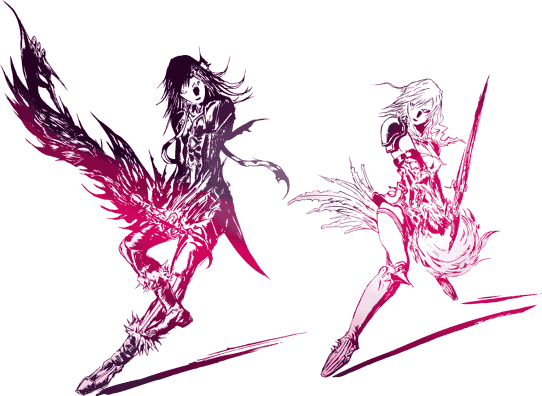
\includegraphics[width=1\columnwidth]{./art/images/ff13-2.png} \end{center}
%
\vspace{0.5cm}
%
Combat takes place in a series of \textbf{rounds} (shortened~\textbf{r}) that take 10 seconds of in-game time each.
Each participant takes one \textbf{turn} per round according to the turn order, which is determined  
through an \mbox{\textbf{initiative check}} at the start of each battle.
Every combatant rolls 2d and the higher their result, the earlier they are placed in this order.
The GM resolves equal results and once determined, the turn order does not change until the end of the battle.
During your turn you can, in any order, move a distance of your AGI+1 units and take an action.
%
\vfill
%
\subsubsection*{Attributes}
Combat proficiencies are determined by the following 7 numerical attributes.
Whenever a calculation results in a non-integer value, the result is always rounded down.
%
\begin{description}[leftmargin=*]
	\item[\large\color{accent} \raisebox{-.2\height}{
\includegraphics[height=0.9\baselineskip]{./art/icons/hp.png}} Hit Points (HP)] increase your durability.
	You have a maximum and a current number of HP, if your current HP falls to 0 you fall unconscious.
	
	\item[\large\color{accent} \raisebox{-.2\height}{
\includegraphics[height=0.9\baselineskip]{./art/icons/mp.png}} Mana Points (MP)] are the resource required for using abilities such as Magic and Techs.
	Similar to HP, you have a maximum and a current number of MP.
	
	\item[\large\color{accent} \raisebox{-.2\height}{
\includegraphics[height=0.9\baselineskip]{./art/icons/str.png}} Strength (STR)] increases the damage dealt by your physical attacks.
	
	\item[\large\color{accent} \raisebox{-.2\height}{
\includegraphics[height=0.9\baselineskip]{./art/icons/def.png}} Defense (DEF)] increases your resilience against physical attacks.
	
	\item[\large\color{accent} \raisebox{-.2\height}{
\includegraphics[height=0.9\baselineskip]{./art/icons/mag.png}} Magic (MAG)]  increases the potency of your healing and attacking spells.
	
	\item[\large\color{accent} \raisebox{-.2\height}{
\includegraphics[height=0.9\baselineskip]{./art/icons/res.png}} Resistance (RES)] increases your resilience against magical attacks.
	
	\item[\large\color{accent} \raisebox{-.2\height}{
\includegraphics[height=0.9\baselineskip]{./art/icons/mov.png}} Agility (AGI)] allows you to evade physical attacks and determines how quickly you can move.
\end{description}

\pagebreak

\subsubsection*{\hypertarget{action}{Actions}}
Below is a list of combat actions, but the GM may allow any other action that can be completed in one turn:
\begin{description}[leftmargin=*]	
	\item[\large\color{accent} \raisebox{-.2\height}{
\includegraphics[height=\baselineskip]{./art/icons/attack.png}} \textbf{Attack}:]  
	You attack an enemy with your weapon. 
	He may evade by passing an \textbf{evasion check} with a DC of 12 minus his AGI. 
	If he fails the check, you reduce the target's HP by your weapon's DMG plus your STR.
	If the evader rolls a 2, you make a \mbox{\textbf{critical hit}}, doubling your usual damage. 
	If he rolls a 12, not only does your Attack miss, but the evader makes an Attack action on you instead, which you cannot evade.
	
	\item[\large\color{accent}  \raisebox{-.2\height}{
\includegraphics[height=\baselineskip]{./art/icons/magic.png}} \textbf{Magic}:] 
	You cast a spell by spending MP, choosing a target within its range and \mbox{\textbf{concentrating}} for a duration.
	While concentrating, you cannot take actions or evade Attacks. 
	After the cast time is up, the spell's effect occurs on the target right \textbf{before your turn} and cannot be evaded even if you are not in range anymore.
	If the spell deals damage or restores HP, add your MAG to the amount.
	Every spell's description has information on its cast time, MP cost, target, range and effect.
	
	\item[\large\color{accent}  \raisebox{-.2\height}{
\includegraphics[height=\baselineskip]{./art/icons/tech.png}}  \textbf{Tech}:] 
	You use a non-magical ability. 
	Techs are used the same way as magic, but their damage is not amplified by your attributes. 
	
	\item[\large\color{accent}  \raisebox{-.2\height}{
\includegraphics[height=\baselineskip]{./art/icons/defend.png}}  \textbf{Defend}:] 
	All damage that you receive by \hyperlink{action}{Attacks} until your next turn is halved.
	
	\item[\large\color{accent}  \raisebox{-.2\height}{
\includegraphics[height=\baselineskip]{./art/icons/item.png}}  \textbf{Item}:] 
	You use an Item from your inventory on yourself or someone within 1u. 
\end{description} 
%
\vspace{0.1cm}
%
\subsubsection*{\hypertarget{sabilities}{Special Abilities}}
Apart from Magic and Techs, characters can also learn the following special abilities:
\begin{description}[leftmargin=*]
	\item[\large\color{accent} \raisebox{-.2\height}{
\includegraphics[width=\baselineskip]{./art/icons/passive.png}} \textbf{Passive}:] 
	Effects that are permanently active.
	
	\item[\large\color{accent} \raisebox{-.2\height}{
\includegraphics[width=\baselineskip]{./art/icons/react.png}} \textbf{Reaction}:]
	Allow you to take certain actions on someone else's turn under specific conditions.
\end{description}
%
\vspace{0.4cm}
%
\example{Combat}
{
	Squall (\textcolor{blue}{DEF:4}, \textcolor{ForestGreen}{AGI:2}, \textcolor{Sepia}{RES:1}) 
	and Seifer (\textcolor{red}{STR:6}, \textcolor{Magenta}{MAG:2}) decide to duel.
	Both are wielding a gunblade~(DMG:\textcolor{Plum}{1d}).
	They roll 2d for initiative: Squall rolls 9 and Seifer rolls 10, so Seifer takes the first turn.
	He begins casting "Fire" (DMG:\textcolor{orange}{2d}, Time:1r) by spending 4~MP, choosing Squall as target and concentrating. 
	Then it's Squall's turn, who chooses to Defend.
	It's Seifer's turn again, so Fire takes effect and Squall suffers \mbox{\textcolor{orange}{2d}+\textcolor{Magenta}{2}-\textcolor{Sepia}{1}} damage. 
	Seifer can still take his turn, so he also Attacks. 
	Squall could evade by passing a 
	\mbox{DC 12-\textcolor{ForestGreen}{2}} 
	check, though by rolling 2 he not only fails, but suffers a Critical Hit! 
	Seifer hits him right above the nose with his blade, inflicting 
	\mbox{\textcolor{Plum}{1d}+\textcolor{red}{6}-\textcolor{blue}{4}}
	damage (Defend and Critical Hit cancel each other out) and leaving a scar.
}
%
\pagebreak
%
\subsubsection*{Damage Types} 
All damage dealt has one of the following basic types:
%
\begin{description}[leftmargin=*]
	\item[\accf{Physical}:] damage dealt by Attacks and Techs is usually physical. 
	Whenever you receive physical damage, subtract your DEF from the amount.
	
	\item[\accf{Magical}:] damage dealt by Magic and Items is usually magical. 
	Whenever you receive magical damage, subtract your RES from the amount.
\end{description}
%
\noindent
In addition, damage can have an elemental type, e.g. due to the used weapon or spell.
Combatants can have \textbf{Weaknesses} or \textbf{Resiliences} against these types. 
When resilient, they only suffer half the usual damage and when weak, they suffers double the usual damage. 
%
\vspace{0.3cm}
%
\begin{tcolorbox}[colback=white, left=1pt,top=0pt,right=1pt,bottom=0pt,colframe=accent,tabularx={@{\hspace{-0.2cm}}cp{0.45\columnwidth}|p{0.45\columnwidth}},sharp corners=south, title={\begin{center} \textbf{Elemental Damage Types} \end{center}}] 
	& \textbf{Fire} \hspace*{\fill} \raisebox{-.4\height}{
\includegraphics[width=0.06\columnwidth]{./art/icons/fire.png}} &
	\textbf{Ice} \hspace*{\fill} \raisebox{-.4\height}{
\includegraphics[width=0.06\columnwidth]{./art/icons/ice.png}}  \vspace{0.1cm} \\
	\hline & \textbf{Lightning} \hspace*{\fill} \raisebox{-.4\height}{
\includegraphics[width=0.06\columnwidth]{./art/icons/lightning.png}}  &
	\textbf{Water} \hspace*{\fill} \raisebox{-.4\height}{
\includegraphics[width=0.06\columnwidth]{./art/icons/water.png}} \vspace{0.1cm} \\ 
	\hline & \textbf{Wind} \hspace*{\fill} \raisebox{-.4\height}{
\includegraphics[width=0.06\columnwidth]{./art/icons/wind.png}} &
	\textbf{Earth} \hspace*{\fill} \raisebox{-.4\height}{
\includegraphics[width=0.06\columnwidth]{./art/icons/earth.png}} \vspace{0.1cm} \\
	\hline & \textbf{Holy} \hspace*{\fill} \raisebox{-.4\height}{
\includegraphics[width=0.06\columnwidth]{./art/icons/holy.png}}  &
	\textbf{Dark} \hspace*{\fill} \raisebox{-.4\height}{
\includegraphics[width=0.06\columnwidth]{./art/icons/dark.png}} \vspace{0.1cm} \\
\end{tcolorbox}

\subsubsection*{Distances}
\textbf{Units} (shortened \textbf{u}) are the basis to measure distance, where 1u is roughly 1m or 3ft.
Characters usually occupy a circle of 1u in diameter in top view. 
The following terms are often used to describe effect distances:
%
\begin{description}[leftmargin=*]
	\item[\accf{Range}:] the maximum distance between the center of the caster and the center of the effect. An effect with range \textbf{Self} is centered at the caster, and one with range \textbf{Weapon} has the same range as the used weapon.
	
	\item[\accf{Target}:] the area of the effect as a maximum distance from its center. 
	Unless stated otherwise, everyone fully or partially in the target area is affected, including allies.
	An effect with target \textbf{Single} affects only a single entity.
\end{description}
%
% Range / Distance Illustration	
\begin{figure}[h]
		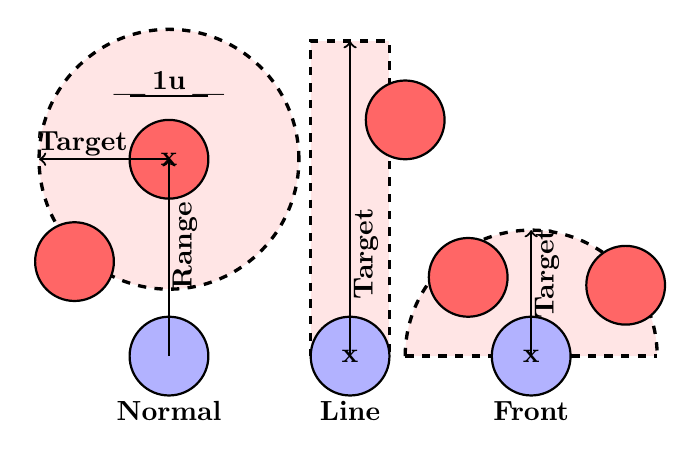
\begin{tikzpicture}[]
		\tikzstyle{test}=[thick, draw, circle, align=center]					
		%Normal
		\node[fill=blue!30!white, test,minimum size = 1cm](caster)at (0,0) {};
		\node[](t2)at (0,-0.7) {\bf Normal};
		\node[fill=red!10!white, test, very thick, dashed ,minimum size = 3.3cm](tarea)at (0,2.5) {};
		\node[fill=red!60!white, test,minimum size = 1cm](target)at (0,2.5) {};
		\node[fill=red!60!white, test,minimum size = 1cm](target)at (-1.2,1.2) {};
		\draw[thick, ->](0,0) -- node[] {}(0,2.5);
		\draw[thick, ->](0,2.5) -- node[] {}(-1.65,2.5);
		\node[rotate=90](t1)at (0.2,1.4) {\bf Range};
		\node[](t2)at (-1.1,2.7) {\bf Target};
		\node[](t3)at (0,2.5) {\bf x};
		\node[](fi)at (-0.5,3.3) {\bf |};
		\node[](se)at (0.5,3.3) {\bf |};
		\draw[thick, -](0.5,3.3) -- node[] {}(-0.5,3.3);
		\node[](sca)at (0,3.5) {\bf 1u};		
		%Line
		\node[draw, fill=red!10!white, rectangle, very thick, dashed ,minimum height = 4cm, minimum width=1cm](tarea)at (2.3,2) {};
		\node[fill=blue!30!white, test,minimum size = 1cm](caster)at (2.3,0) {};
		\node[](t2)at (2.3,-0.7) {\bf Line};
		\node[fill=red!60!white, test,minimum size = 1cm](target)at (3,3) {};
		\draw[thick, ->](2.3,0) -- node[] {}(2.3,4);
		\node[rotate=90](t1)at (2.5,1.3) {\bf Target};
		\node[](t3)at (2.3,0) {\bf x};		
		%Front
		\draw[fill=red!10!white, test, very thick, dashed] (3,0) arc (180:0:1.6cm);
		\draw[dashed, very thick, -](3,0) -- node[] {}(6.2,0);
		\node[fill=blue!30!white, test,minimum size = 1cm](caster)at (4.6,0) {};
		\node[](t2)at (4.6,-0.7) {\bf Front};
		\draw[thick, ->](4.6,0) -- node[] {}(4.6,1.6);
		\node[rotate=90](t1)at (4.8,1.05) {\bf Target};
		\node[fill=red!60!white, test,minimum size = 1cm](target)at (3.8,1) {};
		\node[fill=red!60!white, test,minimum size = 1cm](target)at (5.8,0.9) {};
		\node[](t3)at (4.6,0) {\bf x};
		\end{tikzpicture}
\end{figure}
%
\noindent
The illustration above shows the use of a ranged effect in the normal case and with the two
special target shapes \textbf{Line} and \textbf{Front}.
In situations where you are not able to measure distances accurately, you can also use the following descriptors to give a rough estimate:
%
\pagebreak
%
\begin{description}[leftmargin=*]
	\item[\accf{Adjacent}:] approxmimate distance of 1u or less.
	\item[\accf{Close}:] approxmimate distance between 1u and 3u.
	\item[\accf{Near}:] approxmimate distance between 3u and 6u.
	\item[\accf{Far}:] approxmimate distance of 6u or more.
\end{description}
%
\vfill
\subsubsection*{\hypertarget{status}{Status Effects}}
Status Effects alter your the combat potency in a positive or negative way for a limited duration.
Combatants can suffer multiple different Status Effects at once, but applying the same one twice only refreshes its duration. 
They can also be \textbf{Immune} to certain statuses, meaning they have no effect. 
Below is a list of all Status Effects.
\begin{description}[leftmargin=*]
	
	\item[\large\color{accent} \raisebox{-.2\height}{
\includegraphics[width=\baselineskip]{./art/icons/doom.png}} \textbf{KO}:] 
	You are unconscious and your turns are skipped.
	You suffer KO when your current HP drops to 0 and your HP cannot be increased until this status is removed.  
	Immunity against KO only makes you immune against effects that cause it when above 0 HP.
		
	\item[\large\color{accent} \raisebox{-.1\height}{
\includegraphics[width=\baselineskip]{./art/icons/blind.png}} \textbf{Blind}:] 
	Whenever you \hyperlink{action}{Attack} an enemy, he has \hyperlink{check}{Advantage} on the evasion check.
	
	\item[\large\color{accent} \raisebox{-.1\height}{
\includegraphics[width=\baselineskip]{./art/icons/blink.png}} \textbf{Blink}:] 	
	Whenever you are targeted by an \hyperlink{action}{Attack}, you have \hyperlink{check}{Advantage} on the evasion check.
	
	\item[\large\color{accent} \raisebox{-.1\height}{
\includegraphics[width=\baselineskip]{./art/icons/debrave.png} 
		
\includegraphics[width=\baselineskip]{./art/icons/deprotect.png} 
\includegraphics[width=\baselineskip]{./art/icons/defaith.png} 
		
\includegraphics[width=\baselineskip]{./art/icons/deshell.png}} \textbf{DeATR}:] 
	The according attribute is reduced by 3 (minimum 0), e.g. DeMAG reduces MAG. 
	
	\item[\large\color{accent} \raisebox{-.1\height}{
\includegraphics[width=\baselineskip]{./art/icons/bravery.png} 
		
\includegraphics[width=\baselineskip]{./art/icons/protect.png} 
\includegraphics[width=\baselineskip]{./art/icons/faith.png} 
		
\includegraphics[width=\baselineskip]{./art/icons/shell.png}} \textbf{EnATR}:] 
	The according attribute is increased by 3, e.g. EnMAG increases MAG. 

	\item[\large\color{accent} \raisebox{-.1\height}{
\includegraphics[width=\baselineskip]{./art/icons/immobile.png}} \textbf{Immobile}:] You are unable to move.

	\item[\large\color{accent} \raisebox{-.1\height}{
\includegraphics[width=\baselineskip]{./art/icons/poison.png}} \textbf{Poison}:] 
	You take damage equal to 10\% of your maximum HP at the end of each turn, but cannot fall below 1 HP due to this effect.
	
	\item[\large\color{accent} \raisebox{-.1\height}{
\includegraphics[width=\baselineskip]{./art/icons/silence.png}} \textbf{Silence}:]
	You cannot begin casting \hyperlink{action}{Magic} or using \hyperlink{action}{Techs}, but you can still \hyperlink{action}{Attack}.
	
	\item[\large\color{accent} \raisebox{-.1\height}{
\includegraphics[width=\baselineskip]{./art/icons/stop.png}} \textbf{Sleep}:] 
	Your turns are skipped, but you wake up immediately if you take any damage.
	
	\item[\large\color{accent} \raisebox{-.1\height}{
\includegraphics[width=\baselineskip]{./art/icons/zombie.png}} \textbf{Zombie}:] 
	All healing effects are reversed for you.
	Healing reduces your HP and effects that normally remove KO, inflict it to you instead.	
\end{description} 
%
\vspace*{0.5cm}
%
\example{Status Effects}
{
Noctis and his party fight \hyperlink{malboro}{Malboro}. 
The monster surprises them and uses his Bad Breath ability to inflict multiple Status Effects.
Prompto suffers Sleep and \textcolor{red}{Poison}. 
He cannot move or take actions and before his turn is finished, he loses \textcolor{red}{3} HP, because his maximum HP is 
\textcolor{red}{3}7.
Noctis suffers Silence and \textcolor{Plum}{Blind}.
He cannot use abilities, so he tries to \hyperlink{action}{Attack} Malboro. 
The monster~(AGI:~\textcolor{ForestGreen}{2}) rolls [1,6,4] on the evasion check, barely passing the 
\mbox{DC 12-\textcolor{ForestGreen}{2}} due to \textcolor{Plum}{Advantage}.
}
%
\pagebreak








